%%%%%%%%%%%%%%%%%%%%%%%%%%%%%%%%%%%%%%%%%%%%%%%%%%%%%%%%%%%
%%%%%%%%%%%%%%%%%%%%%%%%%%%%%%%%%%%%%%%%%%%%%%%%%%%%%%%%%%%
%%%%%%%%%%%%%%%%%%%%%%%%%%%%%%%%%%%%%%%%%%%%%%%%%%%%%%%%%%%

%% PREAMBLE! :-)


\documentclass[a4paper, 10pt]{article}

%%% packages - input should be path where your packages.tex file is saved.
%% packages

\usepackage{setspace}

%%%%%%%%%%%%%%%%%%%%%%%%%%%%%%%%%%%%%
\usepackage{sectsty}
\sectionfont{\sffamily\Large}
\subsectionfont{\sffamily}
%%%%%%%%%%%%%%%%%%%%%%%%%%%%%%%%%%%%%
\usepackage[titles]{tocloft}
%%%%%%%%%%%%%%%%%%%%%%%%%%%%%%%%%%%%%

%%% This is a package to use UTF8 CSV files as input and directly convert them to latex tables.
\usepackage{csvsimple}
%https://texblog.org/2012/05/30/generate-latex-tables-from-csv-files-excel/

%%%%%%%%%%%%%%%%%%%%%%%%%%%%%%%%%%%%%
%%%%%%%%%%%%%%%%%%%%%%%%%%%%%%%%%%%%%
%%%%%%%%%%%%%%%%%%%%%%%%%%%%%%%%%%%%%

\usepackage[version=4]{mhchem}
% package for using chemical equations and fonts 
% https://mirror.kumi.systems/ctan/macros/latex/contrib/mhchem/mhchem.pdf

%%%%%%%%%%%%%%%%%%%%%%%%%%%%%%%%%%%%%
%%%%%%%%%%%%%%%%%%%%%%%%%%%%%%%%%%%%%
%%%%%%%%%%%%%%%%%%%%%%%%%%%%%%%%%%%%%

\usepackage{xparse}
% high level user interface package, use with caution
% https://mirror.easyname.at/ctan/macros/latex/contrib/l3packages/xparse.pdf

%%%%%%%%%%%%%%%%%%%%%%%%%%%%%%%%%%%%%
%%%%%%%%%%%%%%%%%%%%%%%%%%%%%%%%%%%%%
%%%%%%%%%%%%%%%%%%%%%%%%%%%%%%%%%%%%%

\usepackage{makeidx}
\usepackage{pdfpages}
\usepackage{lastpage}

%%%%%%%%%%%%%%%%%%%%%%%%%%%%%%%%%%%%%
%%%%%%%%%%%%%%%%%%%%%%%%%%%%%%%%%%%%%
%%%%%%%%%%%%%%%%%%%%%%%%%%%%%%%%%%%%%

%%% Package to control inclusion and exclusion of specific entry in the table of contents.
%%% https://mirror.foobar.to/CTAN/macros/latex/contrib/tocbibind/tocbibind.pdf
\usepackage[nottoc,notlot,notlof]{tocbibind}

%%%%%%%%%%%%%%%%%%%%%%%%%%%%%%%%%%%%%
%%%%%%%%%%%%%%%%%%%%%%%%%%%%%%%%%%%%%
%%%%%%%%%%%%%%%%%%%%%%%%%%%%%%%%%%%%%

\usepackage{bigstrut}
% needed for crazy table commands, its cool trust me!
% https://anorien.csc.warwick.ac.uk/mirrors/CTAN/macros/latex/contrib/multirow/multirow.pdf

%%%%%%%%%%%%%%%%%%%%%%%%%%%%%%%%%%%%%
%%%%%%%%%%%%%%%%%%%%%%%%%%%%%%%%%%%%%
%%%%%%%%%%%%%%%%%%%%%%%%%%%%%%%%%%%%%

\usepackage{graphicx} 								
% Required for the inclusion of images
% https://de.overleaf.com/learn/latex/Inserting_Images

%%%%%%%%%%%%%%%%%%%%%%%%%%%%%%%%%%%%%
%%%%%%%%%%%%%%%%%%%%%%%%%%%%%%%%%%%%%
%%%%%%%%%%%%%%%%%%%%%%%%%%%%%%%%%%%%%

\usepackage{amsmath} 								
% Required for some math elements 
% https://www.namsu.de/Extra/pakete/amsmath/Amsmath.html

%%%%%%%%%%%%%%%%%%%%%%%%%%%%%%%%%%%%%
%%%%%%%%%%%%%%%%%%%%%%%%%%%%%%%%%%%%%
%%%%%%%%%%%%%%%%%%%%%%%%%%%%%%%%%%%%%

\usepackage{amssymb}
% required for some more crazy math elements, checks mal ab!
% http://milde.users.sourceforge.net/LUCR/Math/mathpackages/amssymb-symbols.pdf

%%%%%%%%%%%%%%%%%%%%%%%%%%%%%%%%%%%%%
%%%%%%%%%%%%%%%%%%%%%%%%%%%%%%%%%%%%%
%%%%%%%%%%%%%%%%%%%%%%%%%%%%%%%%%%%%%

%\usepackage{kbordermatrix} 	
% some special matrix-commands						
% http://www.hss.caltech.edu/~kcb/TeX/kbordermatrix.sty
%%%%%%%%%%%%%%%%%%%%%%%%%%%%%%%%%%%%%
%%%%%%%%%%%%%%%%%%%%%%%%%%%%%%%%%%%%%
%%%%%%%%%%%%%%%%%%%%%%%%%%%%%%%%%%%%%

\usepackage{multicol}								
% multicolumn-commands stuffs
% https://de.overleaf.com/learn/latex/Multiple_columns

%%%%%%%%%%%%%%%%%%%%%%%%%%%%%%%%%%%%%
%%%%%%%%%%%%%%%%%%%%%%%%%%%%%%%%%%%%%
%%%%%%%%%%%%%%%%%%%%%%%%%%%%%%%%%%%%%

\usepackage{color}
\definecolor{dkgreen}{rgb}{0,0.6,0}
\definecolor{gray}{rgb}{0.5,0.5,0.5}
\definecolor{mauve}{rgb}{0.58,0,0.82}
\definecolor{darkblue}{rgb}{0.0,0.0,0.6}
\definecolor{cyan}{rgb}{0.0,0.6,0.6}

%%%%%%%%%%%%%%%%%%%%%%%%%%%%%%%%%%%%%
%%%%%%%%%%%%%%%%%%%%%%%%%%%%%%%%%%%%%
%%%%%%%%%%%%%%%%%%%%%%%%%%%%%%%%%%%%%

% package to more precisely wrap your document around ur figure!
% https://de.overleaf.com/learn/latex/wrapping_text_around_figures
\usepackage{wrapfig}								

%%%%%%%%%%%%%%%%%%%%%%%%%%%%%%%%%%%%%
%%%%%%%%%%%%%%%%%%%%%%%%%%%%%%%%%%%%%
%%%%%%%%%%%%%%%%%%%%%%%%%%%%%%%%%%%%%

% the package for bold math symbol commands!
% https://anorien.csc.warwick.ac.uk/mirrors/CTAN/macros/latex/required/tools/bm.pdf
\usepackage{bm}

%%%%%%%%%%%%%%%%%%%%%%%%%%%%%%%%%%%%%
%%%%%%%%%%%%%%%%%%%%%%%%%%%%%%%%%%%%%
%%%%%%%%%%%%%%%%%%%%%%%%%%%%%%%%%%%%%

% subcaption package dependant on caption package (self-explanatory)
% https://www.namsu.de/Extra/pakete/Subcaption.html

\usepackage{caption}
\usepackage{subcaption}

%%%%%%%%%%%%%%%%%%%%%%%%%%%%%%%%%%%%%
%%%%%%%%%%%%%%%%%%%%%%%%%%%%%%%%%%%%%
%%%%%%%%%%%%%%%%%%%%%%%%%%%%%%%%%%%%%

%package for appendix control
% https://mirror.easyname.at/ctan/macros/latex/contrib/appendix/appendix.pdf
\usepackage[toc,page]{appendix}

%%%%%%%%%%%%%%%%%%%%%%%%%%%%%%%%%%%%%
%%%%%%%%%%%%%%%%%%%%%%%%%%%%%%%%%%%%%
%%%%%%%%%%%%%%%%%%%%%%%%%%%%%%%%%%%%%

% This is the listings package to make code appear like actual code!
% https://mirror.foobar.to/CTAN/macros/latex/contrib/listings/listings.pdf
\usepackage{listings}{
 \lstset{frame=tb,
  basicstyle=\fontsize{9}{13}\selectfont\sffamily,
  frame=single,	 
  language=Python,
  breaklines=true,
  showstringspaces=false,
  columns=flexible,
  numbers=left,
  commentstyle=\color{dkgreen},
  stringstyle=\color{mauve},
  tabsize=2
}

%%%%%%%%%%%%%%%%%%%%%%%%%%%%%%%%%%%%%
%%%%%%%%%%%%%%%%%%%%%%%%%%%%%%%%%%%%%
%%%%%%%%%%%%%%%%%%%%%%%%%%%%%%%%%%%%%

% this package for more elaborate appendix commands!
% http://mirror.ox.ac.uk/sites/ctan.org/macros/latex/contrib/appendix/appendix.pdf
\usepackage[toc,page]{appendix}
%\renewcommand{\appendixpagename}{\appendixname}
%\renewcommand{\appendixtocname}{\appendixname}

%%%%%%%%%%%%%%%%%%%%%%%%%%%%%%%%%%%%%
%%%%%%%%%%%%%%%%%%%%%%%%%%%%%%%%%%%%%
%%%%%%%%%%%%%%%%%%%%%%%%%%%%%%%%%%%%%

% this is the hyperlink references package! To make stuff in your text clickable and send you to the right page, URL's, E-mails etc..
% http://mirror.ox.ac.uk/sites/ctan.org/macros/latex/contrib/hyperref/doc/manual.pdf
\usepackage[
    bookmarks,
    bookmarksopen=true,
    colorlinks=true,			% diese Farbdefinitionen zeichnen Links im PDF farblich aus
    linkcolor=black, 			% einfache interne Verknüpfungen
    anchorcolor=black,			% Ankertext
    citecolor=black, 			% Verweise auf Literaturverzeichniseinträge im Text
    filecolor=magenta, 			% Verknüpfungen, die lokale Dateien öffnen
    menucolor=red, 				% Acrobat-Menüpunkte
    urlcolor=blue,				% URL color of course :P
    plainpages=false,		 	% zur korrekten Erstellung der Bookmarks
    pdfpagelabels, 				% zur korrekten Erstellung der Bookmarks
    hypertexnames=true, 		% zur korrekten Erstellung der Bookmarks
    %linktocpage 				% Seitenzahlen anstatt Text im Inhaltsverzeichnis verlinken
]{hyperref}

\usepackage{tcolorbox}
%Fancy boxes around text!
%%%%%%%%%%%%%%%%%%%%%%%%%%%%%%%%%%%%%





%%% Settings!
%% settings
%change relevant macros like title, names etc.

\newcommand{\firstauthorfirstname}{Camilo }
\newcommand{\firstauthorlastname}{Tello Fachin }

\newcommand{\secondauthorfirstname}{Paul Genest }
\newcommand{\secondauthorlastname}{Author }

\newcommand{\doctitle}{PDE Constrained Shape Optimization}

\makeindex
%%%%%%%%%%%%%%%%%%%%%%%%%%%%%%%%%%%%%%%%%%%%%%%%%%%%%%%%%%%%%%%%%%%%%%%%%
%%%%%%%%%%%%%%%%%%%%%%%%%%%%%%%%%%%%%%%%%%%%%%%%%%%%%%%%%%%%%%%%%%%%%%%%%
%%%%%%%%%%%%%%%%%%%%%%%%%%%%%%%%%%%%%%%%%%%%%%%%%%%%%%%%%%%%%%%%%%%%%%%%%

% set the margins of the document, single first input generates evenly spaced margins of that value
\usepackage[margin=2.5cm]{geometry}

%%%%%%%%%%%%%%%%%%%%%%%%%%%%%%%%%%%%%%%%%%%%%%%%%%%%%%%%%%%%%%%%%%%%%%%%%
%%%%%%%%%%%%%%%%%%%%%%%%%%%%%%%%%%%%%%%%%%%%%%%%%%%%%%%%%%%%%%%%%%%%%%%%%
%%%%%%%%%%%%%%%%%%%%%%%%%%%%%%%%%%%%%%%%%%%%%%%%%%%%%%%%%%%%%%%%%%%%%%%%%

\usepackage[utf8]{inputenc}
% u need this one to compile ä ö ü while babel-package is disabled!(english document)!!
% https://www.namsu.de/Extra/pakete/Inputenc.html

%\usepackage[ngerman]{babel}
% uncomment this package to have all the generated text lik TOC and TOC-APP in german
% IF U UNCOMMENT THIS, PUT THE UTF8 INPUTENC PACKAGE IN COMMENT
% https://www.namsu.de/Extra/pakete/German.html

%%%%%%%%%%%%%%%%%%%%%%%%%%%%%%%%%%%%%%%%%%%%%%%%%%%%%%%%%%%%%%%%%%%%%%%%%
%%%%%%%%%%%%%%%%%%%%%%%%%%%%%%%%%%%%%%%%%%%%%%%%%%%%%%%%%%%%%%%%%%%%%%%%%
%%%%%%%%%%%%%%%%%%%%%%%%%%%%%%%%%%%%%%%%%%%%%%%%%%%%%%%%%%%%%%%%%%%%%%%%%


% header and footer settings
% to look up stuff on it go visit this one:
% https://en.wikibooks.org/wiki/LaTeX/Customizing_Page_Headers_and_Footers

\usepackage{fancyhdr}
\setlength{\headheight}{22.25pt}

\renewcommand{\headrulewidth}{0.5pt}
\renewcommand{\footrulewidth}{0.5pt}

\pagestyle{fancy}


% header inputs
\lhead[even output]{Computational Mathematics}
\chead[even output]{Seminary}
\rhead[even output]{
\includegraphics[width=0.8cm]{figures/uni_header}}


%footer inputs
\lfoot[even output]{CSE - SS22}
\cfoot[even output]{Page  \thepage}
\rfoot[even output]{\today}

%%%%%%%%%%%%%%%%%%%%%%%%%%%%%%%%%%%%%%%%%%%%%%%%%%%%%%%%%%%%%%%%%%%%%%%%%
%%%%%%%%%%%%%%%%%%%%%%%%%%%%%%%%%%%%%%%%%%%%%%%%%%%%%%%%%%%%%%%%%%%%%%%%%
%%%%%%%%%%%%%%%%%%%%%%%%%%%%%%%%%%%%%%%%%%%%%%%%%%%%%%%%%%%%%%%%%%%%%%%%%


%settings for PDF metadata, available if rightclick on pdf in adobe and chose properties!

\hypersetup{pdfinfo={
Title={\doctitle},
Subject={Computational Mathematics Seminary},
Author={Camilo Tello Fachin, Paul Genest},
Keywords={Shape Optimization, }{NGSolve, }{Python, }{Finite Element Method, }{CSE}
}}

%%%%%%%%%%%%%%%%%%%%%%%%%%%%%%%%%%%%%%%%%%%%%%%%%%%%%%%%%%%%%%%%%%%%%%%%%
%%%%%%%%%%%%%%%%%%%%%%%%%%%%%%%%%%%%%%%%%%%%%%%%%%%%%%%%%%%%%%%%%%%%%%%%%
%%%%%%%%%%%%%%%%%%%%%%%%%%%%%%%%%%%%%%%%%%%%%%%%%%%%%%%%%%%%%%%%%%%%%%%%%

%% This is the bibliography package,
\usepackage[
backend=bibtex,
style=ieee,
sorting=ynt,
backref=false,
hyperref=true
]{biblatex}

%%%%%%%%%%%%%%%%%%%%%%%%%%%%%%%%%%%%%%%%%%%%%%%%%%%%%%%%%%%%%%%%%%%%%%%%%
%%%%%%%%%%%%%%%%%%%%%%%%%%%%%%%%%%%%%%%%%%%%%%%%%%%%%%%%%%%%%%%%%%%%%%%%%
%%%%%%%%%%%%%%%%%%%%%%%%%%%%%%%%%%%%%%%%%%%%%%%%%%%%%%%%%%%%%%%%%%%%%%%%%

%%% This is an important setting which lets u control the spacing between lines! Just comment/uncomment the desired ones!


%\singlespacing

\onehalfspacing

%\doublespacing






%%% macros - where u define ur macros and newcommands!
% useful macros!


% insert a blank page which is still counted
\newcommand{\blankpage}{
\newpage
\thispagestyle{empty}
\mbox{}
\newpage
}

%%% the bibliohraphy! the settings to the bibliography are changed in the packages.tex file, where the bibtex package is loaded!
\addbibresource{content/04_bibliography.bib}

\begin{document}

%%%%%%%%%%%%%%%%%%%%%%%%%%%%%%%%%%%%%%%%%%%%%%%%%%%%%%%%%%%
%%%%%%%%%%%%%%%%%%%%%%%%%%%%%%%%%%%%%%%%%%%%%%%%%%%%%%%%%%%
%%%%%%%%%%%%%%%%%%%%%%%%%%%%%%%%%%%%%%%%%%%%%%%%%%%%%%%%%%%
          

\begin{titlepage}

\newcommand{\HRule}{\rule{\linewidth}{0.5mm}} % Defines a new command for the horizontal lines, change thickness here

\center % Center everything on the page
 
%----------------------------------------------------------------------------------------
%	HEADING SECTIONS
%----------------------------------------------------------------------------------------

\textsc{\LARGE Vienna University of Technology}\\[1.5cm] % Name of your university/college
\textsc{\Large Computational Mathematics - Seminary}\\[0.5cm] % Major heading such as course name
\textsc{\large Institute of Analysis and Scientific Computing }\\[0.5cm] % Minor heading such as course title

%----------------------------------------------------------------------------------------
%	TITLE SECTION
%----------------------------------------------------------------------------------------

\HRule \\[0.5cm]
{ \huge \bfseries \doctitle}\\[1mm] % Title of your document
\HRule \\[0.5cm]
 
%----------------------------------------------------------------------------------------
%	AUTHOR SECTION
%----------------------------------------------------------------------------------------

\begin{minipage}{0.4\textwidth}
\begin{flushleft} \large
\emph{Authors:}\\
Camilo \textsc{Tello Fachin}\\
12127084 \\
\vspace{3mm}
Paul \textsc{Genest}\\
12131124 \\

\end{flushleft}
\end{minipage}
~
\begin{minipage}{0.4\textwidth}
\begin{flushright} \large
\emph{Supervisor:} \\
Dr. Kevin\textsc{Sturm} \\ % Supervisor's Name
\end{flushright}
\end{minipage}\\[1.5cm]

% If you don't want a supervisor, uncomment the two lines below and remove the section above
%\Large \emph{Author:}\\
%John \textsc{Smith}\\[3cm] % Your name

%----------------------------------------------------------------------------------------
%	DATE SECTION
%----------------------------------------------------------------------------------------

{\large \today}\\[1.5cm] % Date, change the \today to a set date if you want to be precise

%----------------------------------------------------------------------------------------
%	LOGO SECTION
%----------------------------------------------------------------------------------------
\vfill


\includegraphics[width=0.75\textwidth]{figures/uni_titlepage}\\[5cm] % Include a department/university logo
 
%----------------------------------------------------------------------------------------

\vfill % Fill the rest of the page with whitespace
\pagenumbering{alph}

\end{titlepage} 

%\blankpage

% this is to remove the first paragraph sentence indentation! if you want indentation, set the second input to the desired indendation value.
\setlength{\parindent}{0pt}

% this file is loaded, to include PDF's such as declaration of intent for theses, abstracts and summaries in other languages.
\pagenumbering{roman}

\section*{Zusammenfassung}
Zusammenfassung in Deutsch!

\pagebreak

\section*{Abstract}
Abstract in English!




%%% If your TOC is too large for one page, you can distribute it over 2 pages and comment this /blankpage command below! To better control the distribution of the content of the table of content, use the geometry settings and adjust the top and bottom margin for the table of content in the next part of this code.

%\blankpage



%%% Here u define the TOC, a newgeometry command is used to let you design your own TOC margins. just comment out the \newgeometry and the \restoregeometry
%%% command to force the same margins as the rest of the document to the TOC

\pagebreak
\thispagestyle{empty}
\newgeometry{top=2.25cm, bottom=2.25cm}
\tableofcontents
\thispagestyle{empty}
\restoregeometry
\pagebreak
\blankpage

\pagenumbering{arabic}



%%%%%%%%%%%%%%%%%%%%%%%%%%%%%%%%%%%%%%%%%%%%%%%%%%%%%%%%%%%
%%%%%%%%%%%%%%%%%%%%%%%%%%%%%%%%%%%%%%%%%%%%%%%%%%%%%%%%%%%
%%%%%%%%%%%%%%%%%%%%%%%%%%%%%%%%%%%%%%%%%%%%%%%%%%%%%%%%%%%
%%%%%%%%%%%%%%%%%%%%%%%%%%%%%%%%%%%%%%%%%%%%%%%%%%%%%%%%%



%%% This is a first surrogate chapter to intuitively show you how and where to include new chapters!
\section*{Post-Processing}


\begin{figure}[ht]
    \centering
    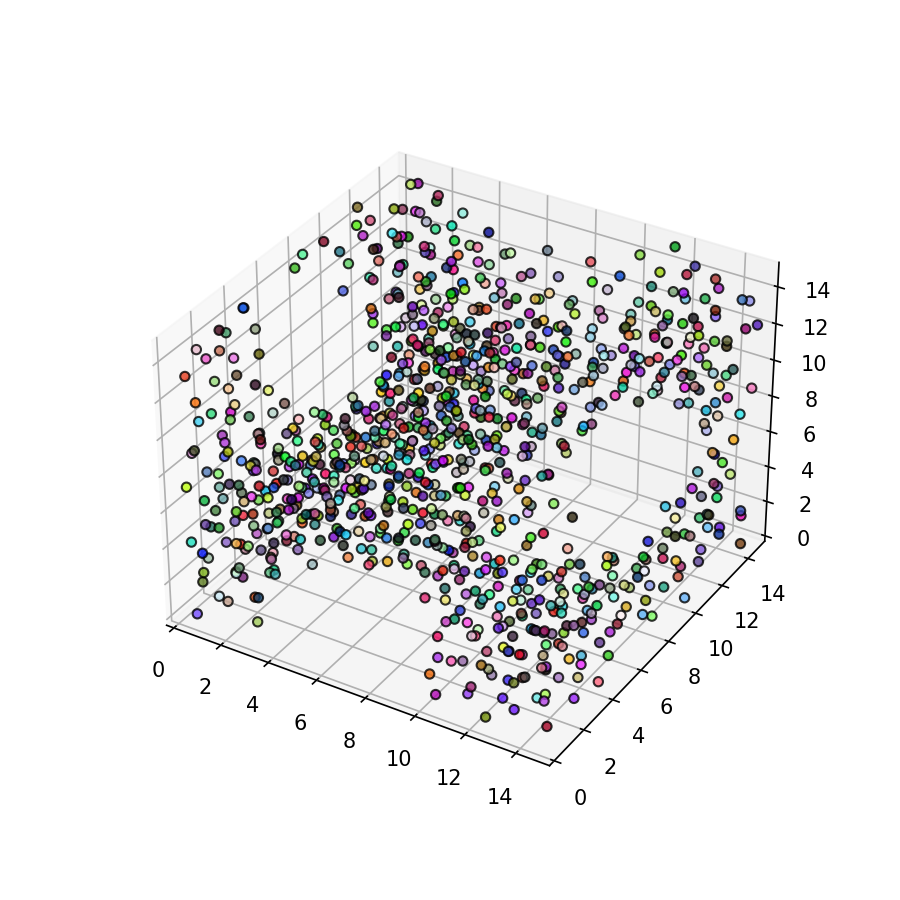
\includegraphics[width=1\textwidth]{figures/3d_plot_IC.png}
	\caption{Initial Condition for Molecular Dynamics Simulation with 1000 Particles at 300K}
	\label{3d_plot_IC}
\end{figure}

Figure \ref{3d_plot_IC} shows the initial condition which is generated from \texttt{ task2.py}. The positions are at a local minimum which is numerically obtained
by the \texttt{scipy.optimize.minimize()} funtcion with the conjugate gradient method. The CG method needs the gradient to obtain the minimum which is passed
as an argument to the function. Not visible in the figure above, are the initial velocites which are also randomly assigned to every particle with the \texttt{numpy.random.multivariate.normal()}
function. This initial condition, namely positions and velocities of each particle, are written to a txt file which is interpreted by pythonfile \texttt{task3.py}.
In said file the trajectories of all thsee particles are calculated by integration of Newtons equations of motion, this part is called the velocity verlet algorithm

\pagebreak

\begin{figure}[ht]
    \centering
    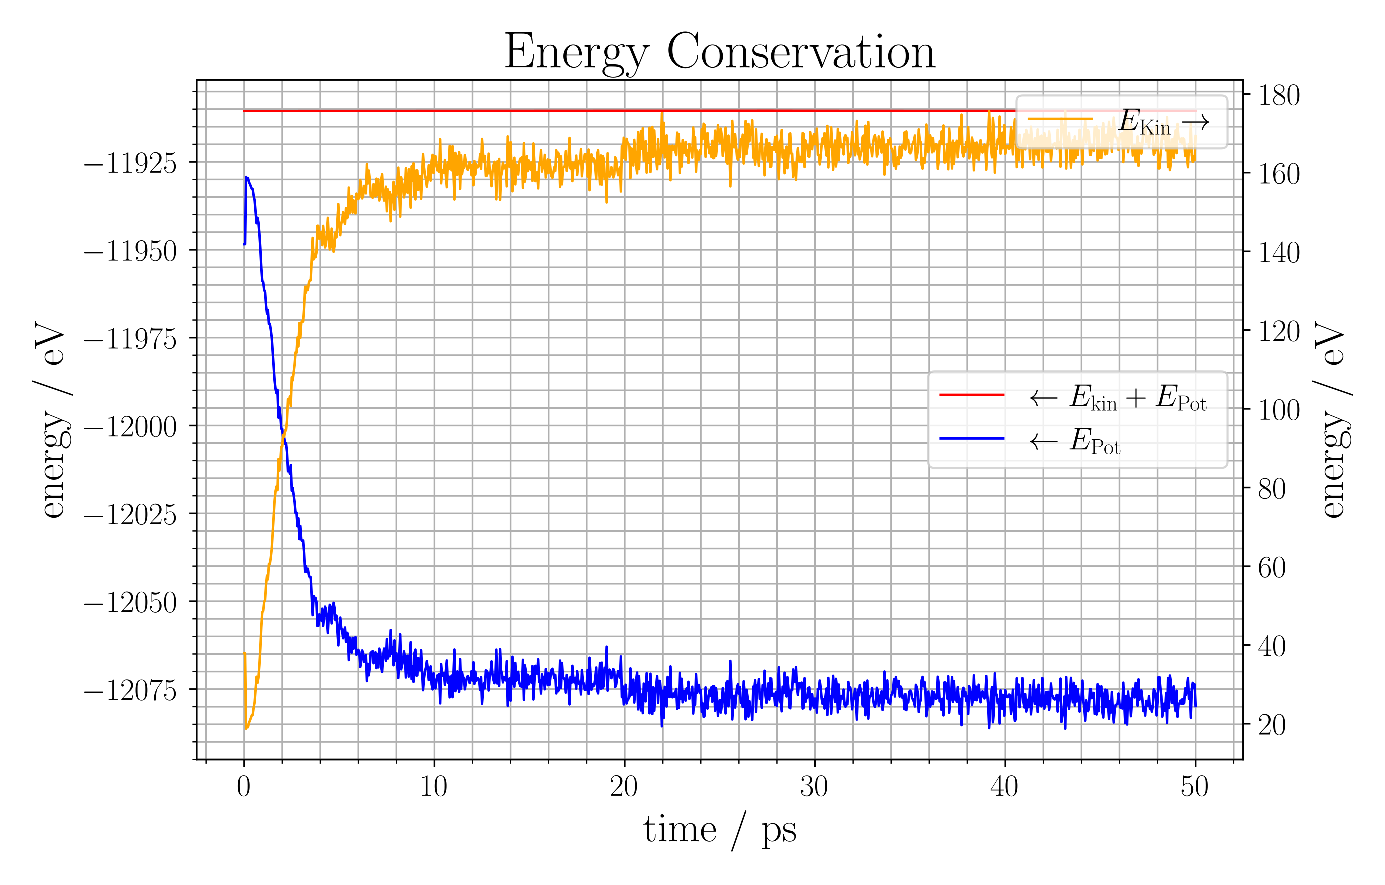
\includegraphics[width=1\textwidth]{figures/energy_conservation.eps}
	\caption{Energy Conservation Plot for $10^6$ timesteps of 0.5 femtoseconds}
	\label{energy_conservation_plot}
\end{figure}

In figure \ref{energy_conservation_plot} above, the energy conservation is shown. Since this molecular dynamics simulation result is obtained numerically,
errors are expected. The main error source being the velocity verlet algorithm, for the chosen timestep, the error is negligible. 
The timestep in this simulation was reduced until a reasonable energy conservation was observed. The timestep chosen was 0.05 femtoseconds. 

\pagebreak

\begin{figure}[ht]
    \centering
    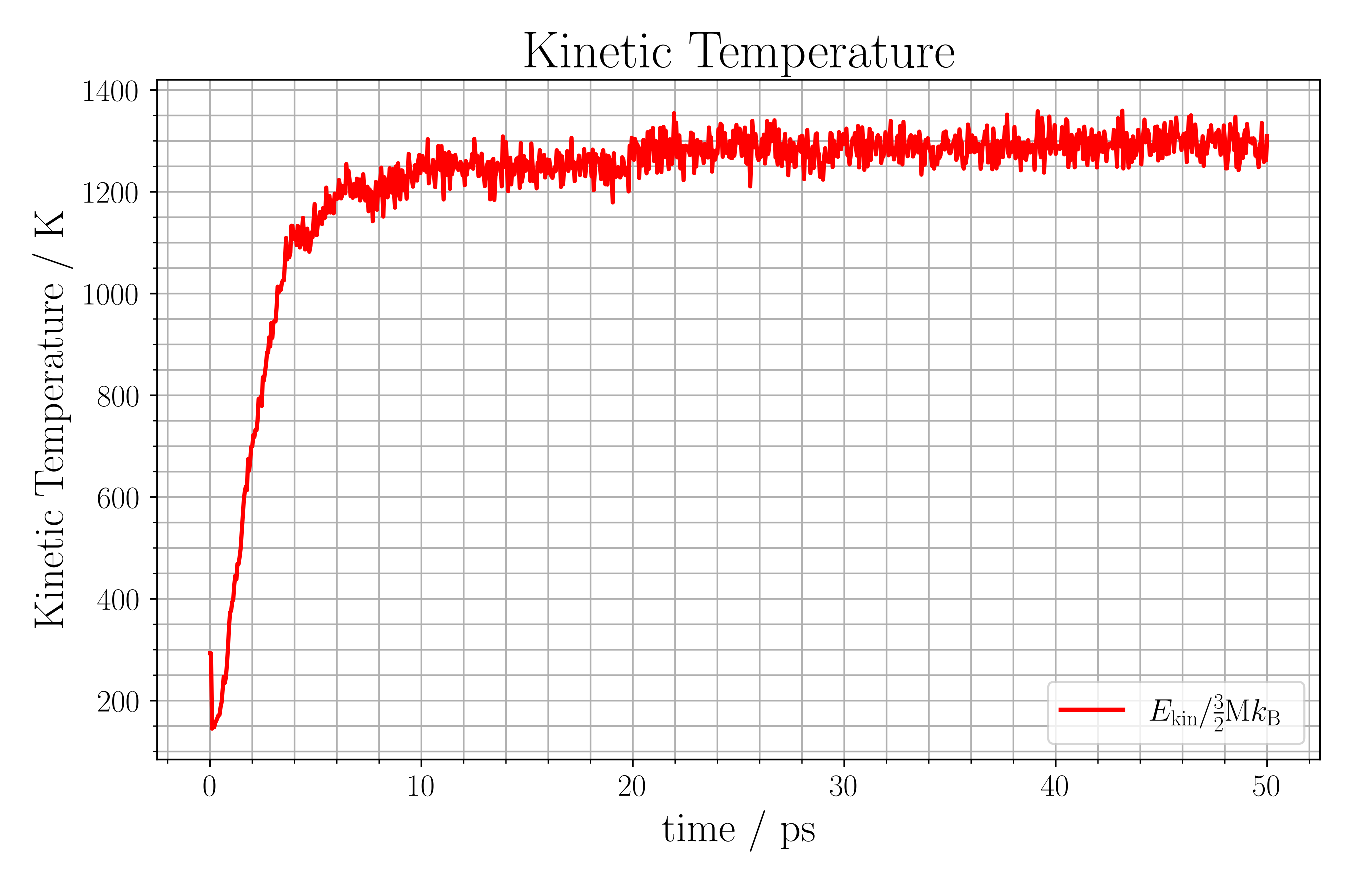
\includegraphics[width=1\textwidth]{figures/kin_temp.eps}
	\caption{Evolution of Kinetic Temperature for $10^6$ timesteps of 0.05 femtoseconds}
	\label{kin_temp_plot}
\end{figure}

In figure \ref{kin_temp_plot} the evolution of the kinetic temperature over the simulated time is plotted. At $t=0$, The kinetic temperature is at 300K, which
is in agreement with the velocities assigned in the initial conditions. The final state where potential and kinetic energy are not changing each other anymore, it reaches a
kinetic temperature of approximately 1300 Kelvin. \\

In order to obtain a specific heat, an approximation formula was provided, where 25 \% of the trajectory data, timewise, had to be neglected.
Said approximation formula yielded a quantity in $\mathrm{J} \slash \mathrm{K}$. If this quantity is divided by the mass of the system,
the weight specifc heat capacity can be obtained. This coefficient is used to model heat transport in solids as well as in fluids,
an example would be the poisson equation.The calculated specific heat capacity was 17.23887287974392 $\mathrm{J} \slash (\mathrm{kg} \cdot \mathrm{K})$. 
A comparable material would be hydrogen with a specific heat capacity of 10.16 $\mathrm{J} \slash (\mathrm{kg} \cdot \mathrm{K})$. However, other than
the equations of motion on the shape of the morse potential function, these simulation results do not have physical meaning.

\pagebreak

%%%%%%%%%%%%%%%%%%%%%%%%%%%%%%%%%%%%%%%%%%%%%%%%%%%%%%%%%%%
%%%%%%%%%%%%%%%%%%%%%%%%%%%%%%%%%%%%%%%%%%%%%%%%%%%%%%%%%%%
%%%%%%%%%%%%%%%%%%%%%%%%%%%%%%%%%%%%%%%%%%%%%%%%%%%%%%%%%%%
%%%%%%%%%%%%%%%%%%%%%%%%%%%%%%%%%%%%%%%%%%%%%%%%%%%%%%%%%

%% During the document writing process, this single .tex file is used to let dasdyou write down a little to do list, just comment it out when the paper is done!
\section*{To Do's}

- What's still to you do make your supervisor/prof happy?
\pagebreak






%%%%%%%%%%%%%%%%%%%%%%%%%%%%%%%%%%%%%%%%%%%%%%%%%%%%%%%%%%%
%%%%%%%%%%%%%%%%%%%%%%%%%%%%%%%%%%%%%%%%%%%%%%%%%%%%%%%%%%%
%%%%%%%%%%%%%%%%%%%%%%%%%%%%%%%%%%%%%%%%%%%%%%%%%%%%%%%%%%%
%%%%%%%%%%%%%%%%%%%%%%%%%%%%%%%%%%%%%%%%%%%%%%%%%%%%%%%%%

%%% Bibliography printing at this point! 
\printbibliography

%%% This is a hardcoded string to enforce it in the table of contents, if you want your "references" string in the TOC to be named differently, such as bibliography or so on, just change the third input to this command below to your desired references naming that should appear in the TOC
\addcontentsline{toc}{section}{References}


%\pagebreak

%%%%%%%%%%%%%%%%%%%%%%%%%%%%%%%%%%%%%%%%%%%%%%%%%%%%%%%%%%%
%%%%%%%%%%%%%%%%%%%%%%%%%%%%%%%%%%%%%%%%%%%%%%%%%%%%%%%%%%%
%%%%%%%%%%%%%%%%%%%%%%%%%%%%%%%%%%%%%%%%%%%%%%%%%%%%%%%%%%%


%%% This is where the appendix .tex file is included, the settings to the appendix are changed in the settings.tex file
\begin{appendix}
\addappheadtotoc
\section{Python Code - PDE Constrained Shape Optimization in \fun{NGSolve}}
\label{app_a}


\begin{lstlisting}[language=Python, title=NGSolve Shape Optimization Code in Python, label=final_code]
from ngsolve import *
from netgen.geom2d import SplineGeometry
from ngsolve.webgui import Draw
import numpy as np
import matplotlib.pyplot as plt

geo = SplineGeometry()
h_coarse = 1
h_fine = 0.15
geo.AddRectangle( (-3,-2), (3, 2), bcs = ("top", "out", "bot", "in"), leftdomain=1, rightdomain=0, maxh=h_coarse) 
geo.AddCircle(c=(0, 0), r=0.6, leftdomain=2, rightdomain=1, bc="outer_cylinder", maxh=h_fine) 
geo.AddCircle(c=(0, 0), r=0.5, leftdomain=0, rightdomain=2, bc="cyl", maxh=h_fine) 
mesh = Mesh(geo.GenerateMesh(maxh=h_coarse))
mesh.Curve(2);
scene1 = Draw(mesh)

# Order of spaces for Taylor-Hood Elements
k = 2
V = H1(mesh,order=k, dirichlet="top|bot|cyl|in|out")
Q = H1(mesh,order=k-1)
FES = FESpace([V,V,Q])

ux,uy,p = FES.TrialFunction()
vx,vy,q = FES.TestFunction()

# stokes equation
def Equation(ux,uy,p,vx,vy,q):
    div_u = grad(ux)[0]+grad(uy)[1] # custom div
    div_v = grad(vx)[0]+grad(vy)[1]
    return (grad(ux)*grad(vx)+grad(uy)*grad(vy) + div_u*q + div_v*p)* dx

a = BilinearForm(FES)
a += Equation(ux,uy,p,vx,vy,q)
a.Assemble()

gfu = GridFunction(FES)
uinf = 0.0005
uin = CoefficientFunction((uinf))
gfu.components[0].Set(uin, definedon=mesh.Boundaries("in|top|bot|out"))

x_velocity = CoefficientFunction(gfu.components[0])
scene_state = Draw(x_velocity, mesh, "vel")

def solveStokes():
    res = gfu.vec.CreateVector()
    res.data = -a.mat * gfu.vec
    inv = a.mat.Inverse(FES.FreeDofs())
    gfu.vec.data += inv * res
    scene_state.Redraw()
solveStokes()

def calc_drag(gfu):
    ux = gfu.components[0]
    uy = gfu.components[1]
    return 0.5*(grad(ux)*grad(ux)+grad(uy)*grad(uy)).Compile()*dx

alpha = 1e-4
surf_t = CoefficientFunction(1)
surf_0 = Integrate(surf_t,mesh)

bc_tx = CoefficientFunction(x)
bc_ty = CoefficientFunction(y)
bc_0x = 1/surf_0*Integrate(bc_tx,mesh)
bc_0y = 1/surf_0*Integrate(bc_ty,mesh)

# Test and trial functions for shape derivate
VEC = H1(mesh, order=2, dim=2, dirichlet="top|bot|in|out")
PHI, X = VEC.TnT()
# gfset denotes the deformation of the original domain and will be updated during the shape optimization
gfset = GridFunction(VEC)
gfset.Set((0,0))
mesh.SetDeformation(gfset)
SetVisualization(deformation=True)

# deformation calculation
gfX = GridFunction(VEC)

ux = gfu.components[0]
uy = gfu.components[1]
p = gfu.components[2]

vol = Parameter(1)
vol.Set(Integrate(surf_t,mesh))

Lagrangian = Equation(ux,uy,p,ux,uy,p) + calc_drag(gfu)  

dJOmega = LinearForm(VEC)
# automatic shape differentiation
dJOmega += Lagrangian.DiffShape(X)

# volume side constraint
vol = Parameter(1)
vol.Set(Integrate(surf_t,mesh))
alpha0 = 1e-4
alpha = Parameter(alpha0)
dJOmega += 2*alpha*(vol-surf_0)*div(X)*dx

# barycenter x sideconstraint
beta0 = 1e-3
beta = Parameter(beta0)
bc_x = Parameter(1)
bc_x.Set((1/surf_0)*Integrate(bc_tx,mesh))
dJOmega += 2*beta*(bc_x-bc_0x)*((1/vol**2)*div(X)*x+(1/vol)*div(X)*x*sum(gfset.vecs[0].data)[0])*dx

# barycenter y sideconstraint
bc_y = Parameter(1)
bc_y.Set((1/surf_0)*Integrate(bc_ty,mesh))
dJOmega += 2*beta*(bc_y-bc_0y)*((1/vol**2)*div(X)*y+(1/vol)*div(X)*y*sum(gfset.vecs[0].data)[1])*dx

b = BilinearForm(VEC)
b += (InnerProduct(grad(X),grad(PHI)+grad(PHI).trans)).Compile() *dx + (InnerProduct(X,PHI)).Compile()*dx

#Cauchy-Riemann Penalisation
gamma0 = 25
gamma = Parameter(gamma0)
zeta = 150
b += zeta*(PHI.Deriv()[0,0] - PHI.Deriv()[1,1])*(X.Deriv()[0,0] - X.Deriv()[1,1])*dx
b += zeta*(PHI.Deriv()[1,0] - PHI.Deriv()[0,1])*(X.Deriv()[1,0] - X.Deriv()[0,1])*dx

def updateParams(v=False):
    vol.Set(Integrate(surf_t,mesh))
    bc_x.Set((1/surf_0)*Integrate(bc_tx,mesh))
    bc_y.Set((1/surf_0)*Integrate(bc_ty,mesh))
    if(v):
        print(vol.Get(), bc_x.Get(), bc_y.Get())
updateParams()

def increaseParams(k=2,v=False):
    alpha.Set(alpha.Get()*k)
    beta.Set(beta.Get()*k)
    gamma.Set(gamma.Get()*k)
    if(v):
        print("alpha: ", alpha.Get(), ", beta: ", beta.Get(), ", gamma: ", gamma.Get())

        def SolveDeformationEquation():
        rhs = gfX.vec.CreateVector()
        rhs.data = dJOmega.vec - b.mat * gfX.vec
        update = gfX.vec.CreateVector()
        update.data = b.mat.Inverse(VEC.FreeDofs()) * rhs
        gfX.vec.data += update

gfset.Set((0,0))
mesh.SetDeformation(gfset)
scene.Redraw()

updateParams()
alpha0 = 1e-4
beta0 = 1e-0
gamma0 = 1e2
alpha.Set(alpha0)
beta.Set(beta0)
gamma.Set(gamma0)

a.Assemble()
solveStokes()

data = [[] for x in range(7)]

iter_max = 800

# try parts of loop
mesh.SetDeformation(gfset)
scene.Redraw()

c = 0

# input("Press enter to start optimization")
for i in range(0,iter_max):
    mesh.SetDeformation(gfset)
    scene.Redraw()
    scene_state.Redraw()
    
    if i%50 == 0:
        print('drag at iteration', i, ': ', Integrate(calc_drag(gfu), mesh))
        
    titles = ["Energy Dissipation","Volume","bc_x","bc_y","scale","gfxnorm","gfxbndnorm"] # collecting data
    data[0].append(Integrate(calc_drag(gfu),mesh))
    data[1].append(vol.Get())
    data[2].append(bc_x.Get())
    data[3].append(bc_y.Get())
    
    a.Assemble()
    solveStokes()
    
    b.Assemble()
    dJOmega.Assemble()
    SolveDeformationEquation()
    updateParams()
    
    mesh.UnsetDeformation()
    
    gfxnorm = Norm(gfX.vec)
    gfxbndnorm = Integrate(sqrt(gfX**2),mesh,BND)
    data[6].append(gfxbndnorm)
    #scale = 0.1 / Norm(gfX.vec)
    scale = 0.01 / gfxnorm
    data[4].append(scale)
    data[5].append(gfxnorm)
    
    
    c += 1
    #if(gfxnorm < 1e-5):
    if(gfxbndnorm < 1e-7 and c > 50):
        if alpha.Get() < 100:
            increaseParams(5,True)
            c = 0
        else:
            print("alpha too big")
            break
            
    gfset.vec.data -= scale * gfX.vec
\end{lstlisting}

\vfill

\end{appendix}


%%%%%%%%%%%%%%%%%%%%%%%%%%%%%%%%%%%%%%%%%%%%%%%%%%%%%%%%%%%
%%%%%%%%%%%%%%%%%%%%%%%%%%%%%%%%%%%%%%%%%%%%%%%%%%%%%%%%%%%
%%%%%%%%%%%%%%%%%%%%%%%%%%%%%%%%%%%%%%%%%%%%%%%%%%%%%%%%%%%


\end{document}

